\documentclass[12pt,a4paper]{article}

% ─── Page Layout ───────────────────────────────────────────────────────────────
\usepackage[a4paper, margin=0.8in, headheight=14pt]{geometry}

% ─── Fonts (XeLaTeX) ───────────────────────────────────────────────────────────
\usepackage{fontspec}
\usepackage{unicode-math}
\setmainfont{TeX Gyre Pagella}
\setmonofont[Scale=0.88]{TeX Gyre Cursor}
\setmathfont{Latin Modern Math}

% ─── Packages ──────────────────────────────────────────────────────────────────
\usepackage{xcolor}
\usepackage{colortbl}
\usepackage{titlesec}
\usepackage{enumitem}
\usepackage{tabularx}
\usepackage{booktabs}
\usepackage{array}
\usepackage{amsmath}
\usepackage{tikz}
\usetikzlibrary{shapes.geometric, arrows.meta, positioning, calc, fit, decorations.pathreplacing}
\usepackage{tcolorbox}
\tcbuselibrary{skins, breakable}
\usepackage{hyperref}
\usepackage{fancyhdr}
\usepackage{graphicx}
\usepackage{microtype}
\hyphenpenalty=10000
\exhyphenpenalty=10000
\sloppy
\usepackage{caption}
\usepackage{setspace}
\usepackage{multirow}
\usepackage{tocloft}

% ─── Q&A helper ────────────────────────────────────────────────────────────────
\newcommand{\Q}[1]{\textbf{#1}\par\noindent\ignorespaces}

% ─── Colour Palette ────────────────────────────────────────────────────────────
\definecolor{myred}{RGB}{196,30,58}
\definecolor{mydark}{RGB}{30,30,50}
\definecolor{mygreen}{RGB}{14,120,80}
\definecolor{myteal}{RGB}{0,130,140}
\definecolor{myamber}{RGB}{180,100,0}
\definecolor{mypurple}{RGB}{100,30,160}
\definecolor{mygray}{RGB}{246,247,249}
\definecolor{mgframe}{RGB}{180,185,200}
\definecolor{watermark}{RGB}{145,150,170}
\definecolor{hdrred}{RGB}{250,232,235}
\definecolor{hdrgreen}{RGB}{220,244,233}
\definecolor{hdrteal}{RGB}{220,242,244}
\definecolor{hdramber}{RGB}{253,242,215}
\definecolor{hdrpurple}{RGB}{238,228,255}
\definecolor{hdrgray}{RGB}{238,240,245}
\definecolor{rowalt}{RGB}{250,251,253}

% ─── Section Formatting ────────────────────────────────────────────────────────
\titleformat{\section}
  {\large\bfseries\color{myred}}{\thesection.}{0.5em}{}
  [\vspace{1pt}{\color{myred}\rule{\linewidth}{0.8pt}}]
\titleformat{\subsection}
  {\normalsize\bfseries\color{myteal}}{\thesubsection}{0.5em}{}
\titlespacing*{\section}{0pt}{18pt}{7pt}
\titlespacing*{\subsection}{0pt}{11pt}{4pt}

% ─── Paragraph ─────────────────────────────────────────────────────────────────
\setlength{\parindent}{0pt}
\setlength{\parskip}{4pt}

% ─── TOC Styling ───────────────────────────────────────────────────────────────
\renewcommand{\cfttoctitlefont}{\large\bfseries\color{myred}}
\renewcommand{\cftaftertoctitle}{\par\noindent{\color{myred}\rule{\linewidth}{0.8pt}}}
\setlength{\cftbeforetoctitleskip}{0pt}
\setlength{\cftaftertoctitleskip}{6pt}
\renewcommand{\cftsecfont}{\normalsize\bfseries\color{mydark}}
\renewcommand{\cftsecpagefont}{\normalsize\bfseries\color{mydark}}
\renewcommand{\cftsecleader}{\cftdotfill{\cftdotsep}}
\setlength{\cftbeforesecskip}{7pt}
\renewcommand{\cftsubsecfont}{\small\color{mydark}}
\renewcommand{\cftsubsecpagefont}{\small\color{mydark}}
\setlength{\cftbeforesubsecskip}{3pt}
\setlength{\cftsubsecindent}{1.4em}

% ─── Table helpers ─────────────────────────────────────────────────────────────
\renewcommand{\arraystretch}{1.45}
\setlength{\tabcolsep}{6pt}
\arrayrulecolor{mydark}
\newcolumntype{B}[1]{>{\small\bfseries\raggedright\arraybackslash}m{#1}}
\newcolumntype{Y}{>{\small\raggedright\arraybackslash}X}
\renewcommand{\tabularxcolumn}[1]{m{#1}}

% ─── Header / Footer ───────────────────────────────────────────────────────────
\pagestyle{fancy}
\fancyhf{}
\fancyhead[L]{\small\color{myred}\textbf{HS-HU601}\;\color{mydark}--- Economics for Engineers}
\fancyhead[R]{\small\color{myteal}\textbf{Module 1 Notes}}
\fancyfoot[C]{\small\color{mydark}\thepage}
\fancyfoot[R]{\small\color{watermark}\textit{\copyright\ Biraj}}
\renewcommand{\headrulewidth}{0.5pt}
\renewcommand{\footrulewidth}{0.3pt}

% ─── Hyperref ──────────────────────────────────────────────────────────────────
\hypersetup{
  colorlinks=true, linkcolor=myteal, urlcolor=myteal,
  pdfauthor={Biraj Sarkar},
  pdftitle={HS-HU601 --- Module 1 Notes}
}

% ─── tcolorbox styles ──────────────────────────────────────────────────────────
\tcbset{
  tikzbox/.style={
    colback=mygray, colframe=mgframe, boxrule=0.6pt, arc=4pt,
    left=8pt, right=8pt, top=6pt, bottom=6pt,
    colbacktitle=mgframe, coltitle=mydark,
    fonttitle=\small\bfseries
  },
  defbox/.style={
    colback=hdrgreen, colframe=mygreen, boxrule=0.8pt, arc=4pt,
    left=9pt, right=9pt, top=6pt, bottom=6pt,
    colbacktitle=mygreen, coltitle=white,
    fonttitle=\small\bfseries
  },
  formulabox/.style={
    colback=hdrteal, colframe=myteal, boxrule=0.8pt, arc=4pt,
    left=9pt, right=9pt, top=7pt, bottom=7pt,
    colbacktitle=myteal, coltitle=white,
    fonttitle=\small\bfseries
  },
  examplebox/.style={
    colback=hdramber, colframe=myamber, boxrule=0.8pt, arc=4pt,
    left=9pt, right=9pt, top=6pt, bottom=6pt,
    colbacktitle=myamber, coltitle=white,
    fonttitle=\small\bfseries
  },
  masonbox/.style={
    colback=hdrpurple, colframe=mypurple, boxrule=0.8pt, arc=4pt,
    left=9pt, right=9pt, top=6pt, bottom=6pt,
    colbacktitle=mypurple, coltitle=white,
    fonttitle=\small\bfseries
  },
  exambox/.style={
    colback=hdrpurple, colframe=mypurple, boxrule=1pt, arc=5pt,
    left=10pt, right=10pt, top=8pt, bottom=8pt,
    colbacktitle=mypurple, coltitle=white,
    fonttitle=\bfseries,
    breakable, title after break={\textbf{Frequently Asked / Viva Questions (contd.)}}}
}
% Make all boxes breakable across pages
\tcbset{breakable}

% ─── TikZ styles ───────────────────────────────────────────────────────────────
\tikzset{
  block/.style={rectangle, draw=myteal, fill=hdrteal,
    text width=2.4cm, align=center, minimum height=0.95cm,
    font=\small, rounded corners=3pt, line width=0.7pt},
  redblock/.style={rectangle, draw=myred, fill=hdrred,
    text width=2.4cm, align=center, minimum height=0.95cm,
    font=\small, rounded corners=3pt, line width=0.7pt},
  netnode/.style={rectangle, draw=myteal, fill=hdrteal,
    text width=1.5cm, align=center, minimum height=0.8cm,
    font=\small, rounded corners=3pt, line width=0.7pt},
  sumjunc/.style={circle, draw=myamber, fill=hdramber,
    minimum size=0.62cm, font=\small, line width=0.8pt},
  snode/.style={circle, draw=mypurple, fill=hdrpurple,
    minimum size=0.55cm, font=\footnotesize, line width=0.7pt},
  arrow/.style={-Stealth, thick, color=mydark},
  redarrow/.style={-Stealth, thick, color=myred},
  line/.style={thick, color=mydark}
}

% ═══════════════════════════════════════════════════════════════════════════════
\begin{document}
% ═══════════════════════════════════════════════════════════════════════════════

\begin{center}
  {\LARGE\bfseries\color{myred} HS-HU601 --- Economics for Engineers}\\[5pt]
  {\normalsize\color{mydark} Semester VI \quad$\bullet$\quad 3L:0T:0P \quad$\bullet$\quad 3 Credits}\\[3pt]
  {\normalsize\color{myteal}\textbf{Module 1 Exam Notes}}\\[3pt]
  {\small\color{mydark} CGEC \;$|$\; B.Tech ECE (2023--27) \;$|$\; \textit{Biraj Sarkar}}
\end{center}
\vspace{2pt}
\noindent{\color{myred}\rule{\linewidth}{1.5pt}}
\vspace{2pt}

\hypersetup{linkcolor=mydark}
\tableofcontents
\hypersetup{linkcolor=myteal}
\newpage

% ===============================================================================
\section{Economic Decision Making}
% ===============================================================================

\begin{tcolorbox}[defbox]
\textbf{Engineering Economics:} A systematic discipline that applies economic principles, techniques, and methodologies to evaluate engineering alternatives. It translates physical engineering designs into financial metrics to determine their feasibility and profitability.
\end{tcolorbox}

\subsection{Overview and Problems}
Engineering problems are solved using two types of criteria:
\begin{enumerate}[label=\textbf{\arabic*.}, leftmargin=*, itemsep=3pt, topsep=2pt]
  \item \textbf{Physical/Technical Criteria:} Assesses whether an alternative is physically feasible (e.g., strength, efficiency, speed, material availability, safety).
  \item \textbf{Economic Criteria:} Assesses whether the alternative is financially viable (e.g., capital cost, rate of return, life-cycle cost, return on investment).
\end{enumerate}

The core problem in engineering economics is the \textbf{allocation of scarce resources} (capital, labor, materials, and time) among competing engineering proposals to achieve maximum economic efficiency.

\subsection{Role of Engineering Economics in Engineering Decisions}
An engineer has a dual role: as a designer/technical expert, and as an economic evaluator. The key roles include:
\begin{itemize}[leftmargin=*, itemsep=2pt]
  \item \textbf{Alternative Selection:} Comparing different designs, processes, or equipment to find the most cost-effective solution.
  \item \textbf{Capital Budgeting:} Evaluating whether a project warrants the investment of company funds.
  \item \textbf{Operational Efficiency:} Identifying opportunities to reduce operating, maintenance, and utility costs.
  \item \textbf{Replacement Decisions:} Determining the optimal time to retire old assets and acquire new ones.
\end{itemize}

\subsection{The Decision-Making Process}
The economic decision-making process is an iterative, structured sequence of steps:

\begin{tcolorbox}[tikzbox, title={The Step-by-Step Economic Decision-Making Process}]
\centering
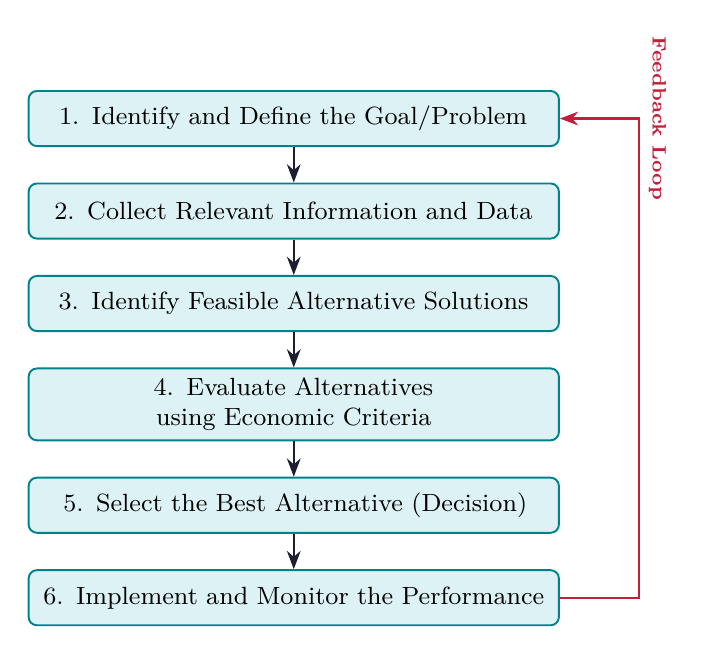
\begin{tikzpicture}[
  stepbox/.style={rectangle, draw=myteal, fill=hdrteal, text width=6.5cm,
    align=center, minimum height=0.7cm, font=\small, rounded corners=3pt, line width=0.7pt},
  flowarrow/.style={-Stealth, thick, color=mydark}
]
  \node[stepbox] (s1) {1. Identify and Define the Goal/Problem};
  \node[stepbox, below=0.45cm of s1] (s2) {2. Collect Relevant Information and Data};
  \node[stepbox, below=0.45cm of s2] (s3) {3. Identify Feasible Alternative Solutions};
  \node[stepbox, below=0.45cm of s3] (s4) {4. Evaluate Alternatives using Economic Criteria};
  \node[stepbox, below=0.45cm of s4] (s5) {5. Select the Best Alternative (Decision)};
  \node[stepbox, below=0.45cm of s5] (s6) {6. Implement and Monitor the Performance};

  \draw[flowarrow] (s1) -- (s2);
  \draw[flowarrow] (s2) -- (s3);
  \draw[flowarrow] (s3) -- (s4);
  \draw[flowarrow] (s4) -- (s5);
  \draw[flowarrow] (s5) -- (s6);

  % Feedback path
  \draw[flowarrow, color=myred] (s6.east) -- ++(1.0,0) |- (s1.east) 
    node[midway, above, rotate=-90, font=\scriptsize\bfseries\color{myred}] {Feedback Loop};
\end{tikzpicture}
\end{tcolorbox}

% ===============================================================================
\section{Engineering Costs and Estimation}
% ===============================================================================

To make sound economic decisions, engineers must understand the different classifications of costs.

\subsection{Fixed and Variable Costs}

\begin{tcolorbox}[defbox]
\textbf{Fixed Costs (FC):} Costs that remain constant in total, independent of the level of output or operational activity within a defined range. 
\par\vspace{3pt}
\textbf{Variable Costs (VC):} Costs that vary in direct proportion to the volume of output or activity level.
\end{tcolorbox}

\begin{tcolorbox}[formulabox, title={\textbf{Total Cost Equation}}]
The total cost ($TC$) for a production volume $q$ is expressed as:
\begin{equation}
  TC(q) = FC + VC(q) = FC + (v \times q)
\end{equation}
Where:
\begin{itemize}[leftmargin=1.5em, itemsep=1pt, topsep=2pt]
  \item[] $FC$ = Total Fixed Cost
  \item[] $VC(q)$ = Total Variable Cost for output $q$
  \item[] $v$ = Variable cost per unit of output
  \item[] $q$ = Quantity produced (output volume)
\end{itemize}
\end{tcolorbox}

\subsection{Marginal and Average Costs}

\begin{tcolorbox}[defbox]
\textbf{Marginal Cost (MC):} The incremental cost incurred by producing one additional unit of output.
\par\vspace{3pt}
\textbf{Average Cost (AC):} The total cost per unit of output produced.
\end{tcolorbox}

\begin{tcolorbox}[formulabox, title={\textbf{Average and Marginal Cost Formulas}}]
For a total cost function $TC(q)$:
\begin{align}
  AC(q) &= \frac{TC(q)}{q} = \frac{FC}{q} + v \\[6pt]
  MC(q) &= \frac{d(TC)}{dQ} \quad \text{(continuous)} \quad \text{or} \quad MC = \frac{\Delta TC}{\Delta q} \quad \text{(discrete)}
\end{align}
\end{tcolorbox}

\subsection{Sunk Costs and Opportunity Costs}

\begin{tcolorbox}[defbox]
\textbf{Sunk Cost:} A cost that has already been incurred in the past and cannot be recovered by any current or future action. Sunk costs are \textbf{irrelevant} for future-oriented decision-making.
\par\vspace{3pt}
\textbf{Opportunity Cost:} The benefit or return forgone (lost) by choosing a specific alternative over the next best alternative. It represents the value of resources in their best alternative use.
\end{tcolorbox}

\begin{tcolorbox}[exambox, title={\textbf{Exam Tip: The Sunk Cost Fallacy}}]
A common error in decision-making is trying to justify continuing an investment or project because "we have already spent so much money on it." In engineering economics, past expenditures are gone. Decisions must be based solely on future cash flows, incremental costs, and benefits.
\end{tcolorbox}

\subsection{Recurring and Nonrecurring Costs}
\begin{itemize}[leftmargin=*, itemsep=3pt]
  \item \textbf{Recurring Costs:} Expenses that occur repeatedly and predictably at regular intervals during the life cycle of an asset (e.g., annual maintenance, insurance, utility bills, raw material purchases).
  \item \textbf{Nonrecurring Costs:} One-time, non-repetitive expenses that occur at specific points, typically at the beginning or end of a project (e.g., initial research and development, land acquisition, equipment purchasing, installation, decommissioning costs).
\end{itemize}

\subsection{Incremental and Life-Cycle Costs}
\begin{itemize}[leftmargin=*, itemsep=3pt]
  \item \textbf{Incremental Cost:} The difference in total cost between two or more feasible alternatives. If Alternative A costs $\$12,000$ and Alternative B costs $\$15,000$, the incremental cost of choosing Alternative B over A is $\$3,000$.
  \item \textbf{Life-Cycle Cost (LCC):} The sum of all costs associated with a product, structure, system, or service over its entire life span. It covers all phases: acquisition, operation, maintenance, and disposal.
\end{itemize}

\subsection{Cash Costs vs. Book Costs}
It is critical to distinguish between transactions that involve real money and those that are purely accounting entries.\par\noindent
\begin{tabularx}{\linewidth}{|B{3.2cm}|Y|Y|}
\hline
\multicolumn{1}{|>{\centering\arraybackslash}m{3.2cm}|}{\textbf{Parameter}} &
\multicolumn{1}{>{\centering\arraybackslash}Y|}{\textbf{\color{myteal}Cash Cost}} &
\multicolumn{1}{>{\centering\arraybackslash}Y|}{\textbf{\color{myamber}Book Cost}} \\
\hline
\textbf{Definition} & Cost that involves an actual cash transaction or out-of-pocket payment. & Cost recorded in accounting books but does not involve a physical cash flow. \\
\hline
\textbf{Examples} & Purchase of raw materials, labor wages, utility bills, rent. & Depreciation of equipment, asset write-downs. \\
\hline
\textbf{Decision Role} & Directly used in economic analysis and cash flow calculations. & Mostly ignored in cash flow analysis (except for their impact on taxes). \\
\hline
\end{tabularx}

% ===============================================================================
\section{Cost Estimation Models}
% ===============================================================================

Cost estimation is the process of predicting the cost of a future engineering project or product.

\subsection{Types of Estimate}
Estimates vary in their detail, accuracy, and timing:
\begin{enumerate}[label=\textbf{\arabic*.}, leftmargin=*, itemsep=3pt, topsep=2pt]
  \item \textbf{Rough / Order-of-Magnitude Estimate:} Done during the initial conceptual phase. Accuracy is low ($\pm 30\%$). Uses historical data and simple scaling factors.
  \item \textbf{Semi-detailed / Budget Estimate:} Prepared during the preliminary design phase when major parameters are defined. Accuracy is moderate ($\pm 15\%$).
  \item \textbf{Detailed / Engineer's Estimate:} Prepared during the final design/bidding phase based on complete specifications and bills of materials. Accuracy is high ($\pm 5\%$).
\end{enumerate}

\subsection{Estimating Models}

\subsubsection{Per-Unit Model}
A simple model where the total cost is estimated by multiplying the number of units by a historical per-unit cost factor.
\begin{equation}
  C = U \times N
\end{equation}
Where $C$ is the total cost, $U$ is the cost per unit (e.g., cost per square foot of building space, cost per mile of highway), and $N$ is the number of units.

\subsubsection{Segmenting Model}
Estimates the total cost by dividing the project into individual components or segments, estimating the cost of each segment separately, and summing them.
\begin{equation}
  C = \sum_{i=1}^{m} C_i
\end{equation}
Where $C_i$ is the cost of segment $i$, and $m$ is the total number of segments. This is a bottom-up estimation technique.

\subsubsection{Cost Index Model}
Adjusts historical costs to present or future costs using cost indices that reflect inflation and changing economic conditions over time.

\begin{tcolorbox}[formulabox, title={\textbf{Cost Index Formula}}]
\begin{equation}
  C_t = C_0 \times \left( \frac{I_t}{I_0} \right)
\end{equation}
Where:
\begin{itemize}[leftmargin=1.5em, itemsep=1pt, topsep=2pt]
  \item[] $C_t$ = Estimated cost at time $t$ (present/future)
  \item[] $C_0$ = Historical cost at reference time $0$ (past)
  \item[] $I_t$ = Cost index value at time $t$
  \item[] $I_0$ = Cost index value at reference time $0$
\end{itemize}
\end{tcolorbox}

\subsubsection{Power-Sizing Model}
Used to estimate the cost of industrial equipment, plants, or facilities of different capacities. It accounts for economies of scale.

\begin{tcolorbox}[formulabox, title={\textbf{Power-Sizing Formula}}]
\begin{equation}
  C_A = C_B \times \left( \frac{S_A}{S_B} \right)^x
\end{equation}
Where:
\begin{itemize}[leftmargin=1.5em, itemsep=1pt, topsep=2pt]
  \item[] $C_A$ = Estimated cost of equipment/facility $A$
  \item[] $C_B$ = Historical cost of equipment/facility $B$
  \item[] $S_A$ = Size or capacity of equipment/facility $A$
  \item[] $S_B$ = Size or capacity of equipment/facility $B$
  \item[] $x$ = Sizing exponent (reflects economies of scale)
\end{itemize}
\par\vspace{4pt}
\textbf{The Six-Tenths Rule:} If the sizing exponent $x$ is unknown, a default value of $x = 0.6$ is often used (applicable to many chemical process reactors, tanks, and pumps).
\begin{itemize}[leftmargin=*, itemsep=2pt, topsep=2pt]
  \item[] $x < 1$: Economies of scale (cost increases slower than capacity).
  \item[] $x = 1$: Linear scaling (no scale advantage).
  \item[] $x > 1$: Diseconomies of scale (cost increases faster than capacity).
\end{itemize}
\end{tcolorbox}

\subsubsection{Improvement and Learning Curve Model}
Reflects the phenomenon where the direct labor hours required to perform a repetitive task decrease as the cumulative number of units produced increases.

\begin{tcolorbox}[formulabox, title={\textbf{Crawford's Learning Curve Model}}]
The time or cost to produce the $N$-th unit, $Z_N$, is given by:
\begin{equation}
  Z_N = K \times N^b
\end{equation}
Where:
\begin{itemize}[leftmargin=1.5em, itemsep=1pt, topsep=2pt]
  \item[] $Z_N$ = Time or cost required to produce the $N$-th unit
  \item[] $K$ = Time or cost required to produce the $1^{\text{st}}$ unit
  \item[] $N$ = Cumulative number of units produced
  \item[] $b$ = Learning exponent (index of learning)
\end{itemize}
\par\vspace{4pt}
The learning exponent $b$ is related to the learning rate $L$ (expressed as a decimal, e.g., $0.80$ for an $80\%$ curve) by:
\begin{equation}
  b = \frac{\log(L)}{\log(2)} = \frac{\ln(L)}{\ln(2)}
\end{equation}
Every time the cumulative production doubles (e.g., from 1 to 2, 2 to 4, 4 to 8), the time to produce that doubled unit is multiplied by the learning rate $L$:
\begin{equation}
  Z_{2N} = L \times Z_N
\end{equation}
\end{tcolorbox}

\subsection{Worked Examples}

\begin{tcolorbox}[examplebox, title={Example 1: Cost Index Model}]
\textbf{Problem:} In 2018, a company installed a heat exchanger at a cost of $\$85,000$. The plant cost index in 2018 was $560$. Estimate the cost of installing an identical heat exchanger in 2026, when the cost index is projected to be $840$.\\[4pt]
\textbf{Solution:}
Identify the given parameters:
\begin{itemize}[leftmargin=*, itemsep=1pt]
  \item[] Reference Cost $C_0 = \$85,000$
  \item[] Reference Index $I_0 = 560$
  \item[] Project Index $I_t = 840$
\end{itemize}
Using the Cost Index formula:
\begin{align*}
  C_{2026} &= C_0 \times \left( \frac{I_t}{I_0} \right) \\[4pt]
  C_{2026} &= 85,000 \times \left( \frac{840}{560} \right) \\[4pt]
  C_{2026} &= 85,000 \times 1.5 \\[4pt]
  C_{2026} &= \$127,500
\end{align*}
\textbf{Answer:} The estimated cost of the heat exchanger in 2026 is \textbf{\$127,500}.
\end{tcolorbox}

\begin{tcolorbox}[examplebox, title={Example 2: Power-Sizing Model}]
\textbf{Problem:} A water treatment plant with a capacity of $2.5$ million gallons per day (MGD) was constructed in 2020 for $\$3.2$ million. Estimate the cost of a similar plant with a capacity of $6.0$ MGD if the power-sizing exponent is $x = 0.68$.\\[4pt]
\textbf{Solution:}
Identify the given parameters:
\begin{itemize}[leftmargin=*, itemsep=1pt]
  \item[] Reference capacity $S_B = 2.5$ MGD, Reference cost $C_B = \$3,200,000$
  \item[] Target capacity $S_A = 6.0$ MGD
  \item[] Sizing exponent $x = 0.68$
\end{itemize}
Using the Power-Sizing formula:
\begin{align*}
  C_A &= C_B \times \left( \frac{S_A}{S_B} \right)^x \\[4pt]
  C_A &= 3,200,000 \times \left( \frac{6.0}{2.5} \right)^{0.68} \\[4pt]
  C_A &= 3,200,000 \times (2.4)^{0.68}
\end{align*}
Calculate the capacity ratio term:
\begin{align*}
  (2.4)^{0.68} &\approx 1.8155 \\[4pt]
  C_A &\approx 3,200,000 \times 1.8155 \\[4pt]
  C_A &\approx \$5,809,600
\end{align*}
\textbf{Answer:} The estimated cost of the 6.0 MGD plant is \textbf{\$5,809,600}.
\end{tcolorbox}

\begin{tcolorbox}[examplebox, title={Example 3: Learning Curve Model}]
\textbf{Problem:} The first prototype of a satellite communications receiver requires $80$ direct labor hours to assemble. The manufacturing line has an estimated learning rate of $85\%$.
\begin{enumerate}[label=\alph*., leftmargin=*, itemsep=2pt, topsep=2pt]
  \item Calculate the learning exponent $b$.
  \item Estimate the labor hours required to assemble the $8^{\text{th}}$ unit.
\end{enumerate}
\textbf{Solution:}
\textbf{(a) Calculate the learning exponent $b$:}
Using the formula $b = \frac{\log(L)}{\log(2)}$ with $L = 0.85$:
\begin{equation*}
  b = \frac{\log(0.85)}{\log(2)} \approx \frac{-0.07058}{0.30103} \approx -0.2345
\end{equation*}

\textbf{(b) Estimate labor hours for the $8^{\text{th}}$ unit ($N = 8$):}
\textit{Method 1: Direct Formula}
\begin{align*}
  Z_8 &= K \times 8^b \\
  Z_8 &= 80 \times 8^{-0.2345} \\
  Z_8 &\approx 80 \times 0.6141 \approx 49.13 \text{ hours}
\end{align*}
\textit{Method 2: Doubling Principle (Verification)}
Since $8$ is a double of $4$, which is a double of $2$, which is a double of $1$:
\begin{align*}
  Z_1 &= 80 \text{ hours} \\
  Z_2 &= 80 \times 0.85 = 68 \text{ hours} \\
  Z_4 &= 68 \times 0.85 = 57.8 \text{ hours} \\
  Z_8 &= 57.8 \times 0.85 = 49.13 \text{ hours}
\end{align*}
Both methods yield identical results.\\[4pt]
\textbf{Answer:} (a) The learning exponent $b$ is \textbf{-0.2345}. (b) The labor hours for the $8^{\text{th}}$ unit is \textbf{49.13 hours}.
\end{tcolorbox}

% ===============================================================================
% MANDATORY QUICK REVISION PAGE
% ===============================================================================
\newpage
\begin{center}
  {\large\bfseries\color{myred} Quick Revision --- Module I}\\[3pt]
  {\small\color{mydark} Introduction \& Cost Estimation $|$ HS-HU601}
\end{center}
\noindent{\color{myred}\rule{\linewidth}{1.2pt}}
\vspace{4pt}

\begin{tcolorbox}[formulabox, title={\textbf{Key Formulas at a Glance}}]
\renewcommand{\arraystretch}{1.3}
\begin{tabularx}{\linewidth}{B{3.8cm} X}
Total Cost              & $TC(q) = FC + VC = FC + (v \times q)$ \\[4pt]
Average Cost            & $AC(q) = \frac{TC(q)}{q} = \frac{FC}{q} + v$ \\[4pt]
Marginal Cost           & $MC(q) = \frac{d(TC)}{dq} \approx \frac{\Delta TC}{\Delta q}$ \\[4pt]
Cost Indexing           & $C_t = C_0 \times \left( \frac{I_t}{I_0} \right)$ \\[6pt]
Power-Sizing            & $C_A = C_B \times \left( \frac{S_A}{S_B} \right)^x$ \quad (six-tenths rule: $x = 0.6$) \\[6pt]
Learning Curve          & $Z_N = K \times N^b$ \\[4pt]
Learning Exponent       & $b = \frac{\log(L)}{\log(2)}$ \quad ($L$ = learning rate as a decimal)
\end{tabularx}
\end{tcolorbox}

\begin{tcolorbox}[defbox, title={\textbf{One-Line Definitions}}]
\begin{itemize}[leftmargin=*, itemsep=2pt, topsep=0pt]
  \item \textbf{Fixed Cost:} Expense that does not change with production output (e.g., rent, insurance).
  \item \textbf{Variable Cost:} Expense that increases or decreases proportionally with output volume (e.g., raw materials).
  \item \textbf{Sunk Cost:} Past expense that cannot be recovered; irrelevant for future decision-making.
  \item \textbf{Opportunity Cost:} The potential benefit lost by choosing one alternative over another.
  \item \textbf{Incremental Cost:} The change in total cost resulting from selecting one alternative over another.
  \item \textbf{Cash Cost:} Cost representing an out-of-pocket transaction involving actual cash flow.
  \item \textbf{Book Cost:} Recorded non-cash expense representing accounting transactions (e.g., depreciation).
  \item \textbf{Life-Cycle Cost:} The sum of all costs (acquisition, O\&M, disposal) over the lifespan of an asset.
\end{itemize}
\end{tcolorbox}

\begin{tcolorbox}[exambox, title={\textbf{Frequently Asked / Viva Questions}}]
\begin{enumerate}[topsep=0pt, label=\textbf{Q\arabic*.}, itemsep=5pt]
  \item \Q{What is the difference between physical and economic feasibility?}
    Physical feasibility ensures an engineering design is mechanically and structurally possible, while economic feasibility ensures it makes financial sense and yields a positive return.
  \item \Q{Why are sunk costs completely ignored in economic decision-making?}
    Sunk costs are historical expenditures that cannot be changed by any present or future choice. Only future incremental cash flows are affected by new decisions.
  \item \Q{Explain opportunity cost with a practical engineering example.}
    Opportunity cost is the profit forgone from an unselected alternative. For example, if a firm uses its warehouse for assembly rather than renting it out for $\$5,000$/month, the opportunity cost of assembly is $\$5,000$/month.
  \item \Q{What is the "six-tenths rule" in cost estimation?}
    The six-tenths rule is an empirical rule stating that the cost of a new facility/equipment of size $S_A$ is estimated as the cost of reference size $S_B$ multiplied by $(S_A/S_B)^{0.6}$.
  \item \Q{What is the difference between cash costs and book costs in engineering accounts?}
    Cash costs require an actual cash outflow (e.g., wages, raw materials). Book costs are accounting entries that do not involve cash flows (e.g., depreciation).
  \item \Q{How does the Crawford learning curve model function?}
    It states that the time to produce the $N$-th unit decreases exponentially according to $Z_N = K \times N^b$. Every time cumulative production doubles, unit labor time decreases by the learning rate.
  \item \Q{What does a power-sizing exponent $x < 1.0$ indicate?}
    It indicates economies of scale, meaning that doubling the capacity of the equipment will result in a cost increase of less than double ($2^x < 2$).
  \item \Q{Why is life-cycle cost (LCC) a better decision metric than initial acquisition cost?}
    An alternative with a lower purchase price may have high operating and maintenance costs. LCC accounts for all costs from acquisition to disposal, preventing long-term deficits.
  \item \Q{Distinguish between recurring and nonrecurring costs.}
    Recurring costs are periodic and repetitive (e.g., annual maintenance, monthly utility bills). Nonrecurring costs are one-time costs (e.g., land purchase, design costs).
  \item \Q{What are the typical accuracy ranges for the three major types of cost estimates?}
    Rough/Order-of-Magnitude estimate has an accuracy of $\pm 30\%$; Semi-detailed/Budget has $\pm 15\%$; and Detailed/Engineer's estimate has $\pm 5\%$.

  \item \Q{What is the sunk cost fallacy, and why is it dangerous in engineering projects?}
    It is the psychological tendency to continue investing in a failing project because of past non-recoverable expenditures, which leads to further losses.
  \item \Q{What are the components of the total cost equation, and how are average and marginal costs derived?}
    Total cost is $TC = FC + v \times q$. Average cost is derived by dividing total cost by quantity ($AC = FC/q + v$). Marginal cost is the derivative of total cost with respect to quantity ($MC = v$ for linear costs).
\end{enumerate}
\end{tcolorbox}

\begin{tcolorbox}[tikzbox, title={Comparison of Cost Estimating Models}]
\renewcommand{\arraystretch}{1.4}
\par\noindent
\begin{tabularx}{\linewidth}{|B{2.3cm}|Y|Y|Y|}
\hline
\textbf{Model Name} & \textbf{Core Formula} & \textbf{Data Needed} & \textbf{Primary Application} \\
\hline
\textbf{Per-Unit} & $C = U \times N$ & Historical unit rate $U$, quantity $N$ & Very early stage construction cost (e.g., cost per sq.\ ft.). \\
\hline
\textbf{Segmenting} & $C = \sum C_i$ & Detailed component cost breakdown & Detailed bottom-up estimates; bill of materials. \\
\hline
\textbf{Cost Index} & $C_t = C_0 \left( \frac{I_t}{I_0} \right)$ & Historical cost $C_0$, historical \& current indices & Adjusting past costs for inflation or price changes over time. \\
\hline
\textbf{Power-Sizing} & $C_A = C_B \left( \frac{S_A}{S_B} \right)^x$ & Size $S$, reference cost $C_B$, exponent $x$ & Estimating industrial equipment/plant capacity cost scaling. \\
\hline
\textbf{Learning Curve} & $Z_N = K \times N^b$ & First unit hours $K$, learning rate $L$ & Estimating labor costs for manufacturing assembly runs. \\
\hline
\end{tabularx}
\end{tcolorbox}

\end{document}
